%----------------------------------------------------------------------------------------
%	PACKAGES AND OTHER DOCUMENT CONFIGURATIONS
%----------------------------------------------------------------------------------------
\documentclass[11pt,fancychapters]{report}
\usepackage[a4paper, total={6in, 8in}]{geometry}
\usepackage{standalone}
\usepackage{listings}
\usepackage{color}
\usepackage{setspace}
\usepackage{hyperref}
\usepackage{acro}
\usepackage{amsmath}
\usepackage{amsthm}
\usepackage{graphicx}
\usepackage{geometry}
\usepackage{subcaption}
\usepackage{cancel}
\usepackage{tikz}
\usepackage{color}
\usetikzlibrary{calc,trees,positioning,arrows,chains,shapes.geometric,%
    decorations.pathreplacing,decorations.pathmorphing,shapes,%
    matrix,shapes.symbols}
\DeclareAcronym{nn}{
	short = NN,
	long = neural network
}

\DeclareAcronym{neta}{
	short = NETA,
	long = net-activation
}

\DeclareAcronym{mse}{
	short = MSE,
	long = mean square error
}

\DeclareAcronym{kNN}{
	short = kNN,
	long = k-nearest neighbor,
}

\DeclareAcronym{sgd}{
	short = SGD,
	long = stochastic gradient descent,
}


\DeclareAcronym{adam}{
	short = adam,
	long = adaptive moment estimation
}

\DeclareAcronym{cnn}{
	short = CNN,
	long = convolutionnal neural network
}

\DeclareAcronym{rnn}{
	short = RNN,
	long = recursive neural network
}
\definecolor{Code}{rgb}{0,0,0}
\definecolor{Decorators}{rgb}{0.5,0.5,0.5}
\definecolor{Numbers}{rgb}{0.5,0,0}
\definecolor{MatchingBrackets}{rgb}{0.25,0.5,0.5}
\definecolor{Keywords}{rgb}{0,0,1}
\definecolor{self}{rgb}{0,0,0}
\definecolor{Strings}{rgb}{0,0.63,0}
\definecolor{Comments}{rgb}{0,0.63,1}
\definecolor{Backquotes}{rgb}{0,0,0}
\definecolor{Classname}{rgb}{0,0,0}
\definecolor{FunctionName}{rgb}{0,0,.7}
\definecolor{Operators}{rgb}{0,0,0}
\definecolor{Background}{rgb}{0.98,0.98,0.98}

\lstdefinestyle{python}{
  numbers=left,
  numberstyle=\footnotesize,
  numbersep=1em,
  xleftmargin=1em,
  framextopmargin=2em,
  framexbottommargin=2em,
  showspaces=false,
  showtabs=false,
  showstringspaces=false,
  frame=l,
  tabsize=4,
  % Basic
  basicstyle=\ttfamily\small\setstretch{1},
  backgroundcolor=\color{Background},
  language=Python,
  % Comments
  commentstyle=\color{Comments}\slshape,
  % Strings
  stringstyle=\color{Strings},
  morecomment=[s][\color{Strings}]{"""}{"""},
  morecomment=[s][\color{Strings}]{'''}{'''},
  % keywords
  morekeywords={import,from,class,def,for,while,if,is,in,elif,else,not,and,or,print,break,continue,return,True,False,None,access,as,,del,except,exec,finally,global,import,lambda,pass,print,raise,try,assert},
  keywordstyle={\color{Keywords}\bfseries},
  % additional keywords
  morekeywords={[2]@invariant},
  keywordstyle={[2]\color{Decorators}\slshape},
  emph={self},
  emphstyle={\color{self}\slshape},
  breaklines=true
}

\geometry{top=1.3in,bottom=1.3in}
\hypersetup{
    colorlinks,
    citecolor=black,
    filecolor=black,
    linkcolor=black,
    urlcolor=black
}

\definecolor{DarkerGreen}{RGB}{0,179,45}

\newtheorem{exmp}{Example}[section]

\newcommand{\codeExample}[2]{
	\begin{exmp}
      #1
      \noindent\begin{minipage}{\linewidth}
      \begin{lstlisting}[style=python]
          #2
      \end{lstlisting}
      \end{minipage}
    \end{exmp}
}

\newcommand\MyLBrace[2]{%
  \left.\rule{0pt}{#1}\right\}\text{#2}}
  
%----------------------------------------------------------------------------------------
%	REPORT
%----------------------------------------------------------------------------------------

\title{ARN_PW3}

\begin{document}

%%%%%%%%%%%%%%%%%%%%%%%%%%%%%%%%%%%%%%%%%
% Uppsala University Assignment Title Page 
% LaTeX Template
% Version 1.0 (27/12/12)
%
% This template has been downloaded from:
% http://www.LaTeXTemplates.com
%
% Original author:
% WikiBooks (http://en.wikibooks.org/wiki/LaTeX/Title_Creation)
% Modified by Olivier D'Ancona to fit HEIG-VD
% License:
% CC BY-NC-SA 3.0 (http://creativecommons.org/licenses/by-nc-sa/3.0/)

%\title{Title page with logo}
%----------------------------------------------------------------------------------------
%	PACKAGES AND OTHER DOCUMENT CONFIGURATIONS
%----------------------------------------------------------------------------------------

\documentclass[12pt]{article}
\usepackage[english]{babel}
\usepackage[utf8x]{inputenc}
\usepackage{amsmath}
\usepackage{graphicx}
\usepackage{float}
\usepackage[colorinlistoftodos]{todonotes}

\begin{document}

\begin{titlepage}

\newcommand{\HRule}{\rule{\linewidth}{0.5mm}} % Defines a new command for the horizontal lines, change thickness here

\center % Center everything on the page
 
%----------------------------------------------------------------------------------------
%	HEADING SECTIONS
%----------------------------------------------------------------------------------------

\textsc{\LARGE Haute École d'Ingénierie et de Gestion du Canton de Vaud}\\[1.5cm] % Name of your university/college

\includegraphics[scale=.2]{images/heig.png}\\[1cm] % Include a department/university logo - this will require the graphicx package
\textsc{\Large Gestion de projet de Machine Learning}\\[0.5cm] % Major heading such as course name
\textsc{\large GML}\\[0.5cm] % Minor heading such as course title


%----------------------------------------------------------------------------------------
%	TITLE SECTION
%----------------------------------------------------------------------------------------

\HRule \\[0.4cm]
{ \huge \bfseries Crapauduc - 2022}\\[0.4cm] % Title of your document
\HRule \\[1.5cm]
 
%----------------------------------------------------------------------------------------
%	AUTHOR SECTION
%----------------------------------------------------------------------------------------

\begin{minipage}{0.4\textwidth}
\begin{flushleft} \large
\emph{Authors:}\\
Schaller \textsc{Joris}\\ % Your name
D'Ancona \textsc{Olivier}\\ % Your name
Logan  \textsc{Victoria}\\ % Your name
Akoumba \textsc{Erica Ludivine}\\ % Your name
Wichoud \textsc{Nicolas}\\ % Your name

\end{flushleft}

\end{minipage}\\[1.5cm]

% If you don't want a supervisor, uncomment the two lines below and remove the section above
%\Large \emph{Author:}\\
%John \textsc{Smith}\\[3cm] % Your name

%----------------------------------------------------------------------------------------
%	DATE SECTION
%----------------------------------------------------------------------------------------

{\large \today}\\[2cm] % Date, change the \today to a set date if you want to be precise

\vfill % Fill the rest of the page with whitespace

\end{titlepage}


\end{document}

\newpage
\pagenumbering{roman}
\tableofcontents
\newpage
\pagenumbering{arabic}

\chapter{Introduction}
Ce projet de machine learning nous a été proposé dans le cadre du cours de Gestion et valorisation de projet en Machine Learning (GML), donné en 5ème du cursus de Bachelor en Informatique spécialisé en ingénierie des données à la HEIG-VD. Le but de ce travail est de nous faire découvrir la gestion et organisation impliquée par un travail de machine learning, autant au niveau de la recherche technologique qu'au niveau de l'organisation d'équipe, notamment au niveau de la distribution de tâches, gestion d'équipe et de délais. \newline

Le projet étudié ici est un projet existant ayant déjà été réalisé plusieurs fois par le professeur et ses étudiant.e.s : l'étude de crapauducs. Un crapauduc est un “petit conduit sous une route, permettant le passage protégé des batraciens” - selon Le Robert. En 2017, dix-huit crapauducs (\textit{Figure 1.1}) ont étés construits le long de la route d'Aubonne à Gimel - canton de Vaud - afin de permettre aux grenouilles, crapauds et tritons de traverser la route des bois à l'étang en toute sécurité. \newline

À l'intérieur de ces crapauducs ont été installée une caméra équipée d'un capteur, qui implique la prise d'une petite série de photos (\textit{Figure 1.2}) lors de la détection de mouvement, ainsi qu'une planche afin de faciliter la distinction des objets du sol. Comptant moins de caméras que de crapauducs, les caméras n'étaient pas rattachée à un crapauduc et comptent donc des images prises depuis différents crapauducs.\newline

\begin{figure}[!htb]
    \centering
    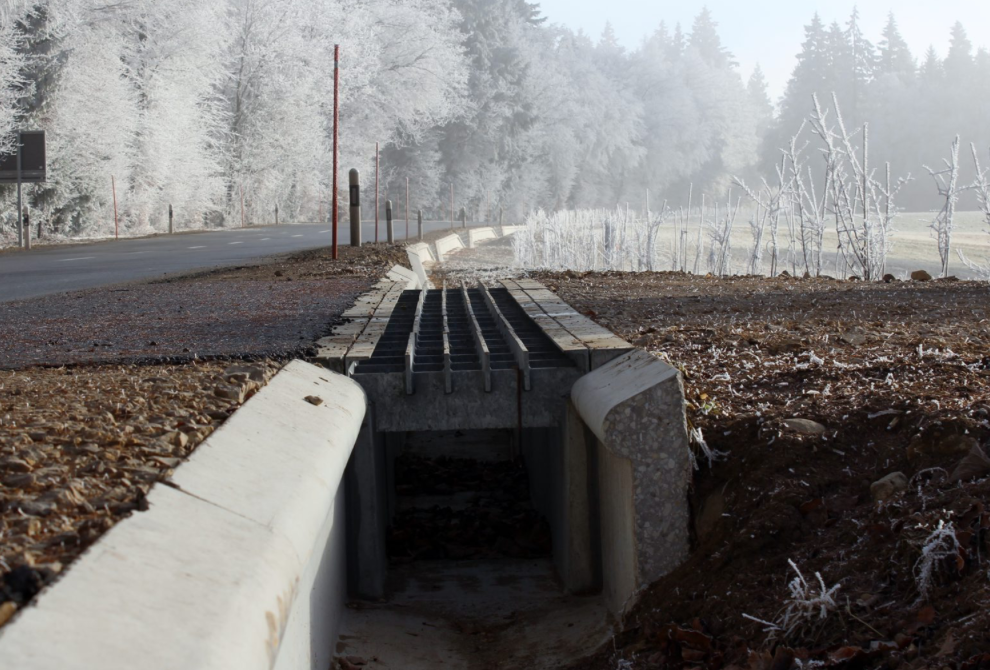
\includegraphics[width=200px]{images/introduction_crapauduc_exterieur.png}
    \caption{Un des 18 crapauducs installés pour l'étude}
    \label{fig:Un des 18 crapauducs installés pour l'étude}
\end{figure}

\newpage

\begin{figure}[!htb]
    \centering
    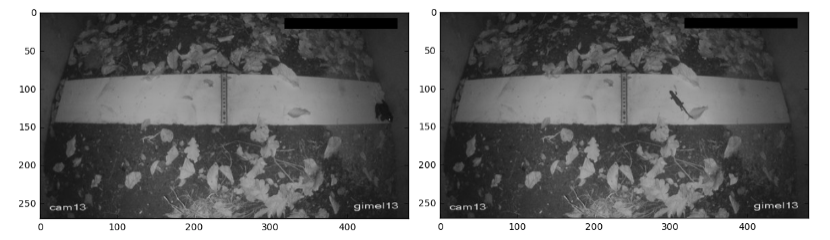
\includegraphics[width=300px]{images/introduction_crapauduc_exemple_prise_camera.png}
    \caption{Exemples des images d'amphibiens prises par les cameras}
    \label{fig:Exemples des images d'amphibiens prises par les cameras}
\end{figure}

 Au terme de la première année d'utilisation, ces voies ont été empruntées par plus de 6'000 crapauds, grenouilles et tritons confondus. Ce comptage a été effectué par des chercheurs, qui ont du regarder les images prises par les caméras et compter les animaux "à la main". Le projet Crapauduc vise ainsi à utiliser l'apprentissage automatique (Machine Learning) pour automatiser le comptage des batraciens. \newline

Notre objectif pour ce projet est donc de détecter la présence ou non de grenouille/crapaud et tritons (en considérant les grenouilles et crapauds comme une seule et même catégorie) en utilisant l'apprentissage automatique. Pour se faire, nous avons les prises des caméras du 23 février 2017 au 20 avril de la même année, totalisant près de 1 million d'images, dont on connaît pour chacune la caméra dont elle provient ainsi que la date (YYYY-MM-DD) et l'heure et minute à laquelle elle a été prise.\newline

Enfin, le professeur nous a également mis à disposition sa labelisation de 2020 de ces images, des bounding box pour certaines images, ainsi que les données météos enregistrées durant cette période (notamment la température, le vent, la précipitation, l'humidité).

\chapter{Context}

\section{Location}

\section{Cameras}


Ceci est un acronyme \acl{kNN}
\chapter{Gestion du projet}
\section{Organisation du projet}
Dès le départ, nous avons décider de travailler avec git, plus précisement 
sur \href{https://github.com}{github}. Nous avons donc créé une organisation afin de séparer les différents dépots. Nous en avons définis 2, mais les membres de l'organisation étaient libres d'en ajouté d'autres.
\begin{itemize}
    \item crapauduc.  Ce dépôt est le dépot principal où les notebooks des modèles sont déposés, nous y avons aussi placé les rapports des anciens étudiants afin d'y avoir un accès rapide. Nous y avons aussi déposé unun subset d'image d'environ 0.5 Gib permettant le fine tuning.
    \item utils. Ce dépôt contient des scripts faisant des transformormations ou des analyses sur les données. Nous y avons par exemple un script qui permet de convertir les annotations de csv à COCO.
\end{itemize}

De plus, nous avons créer un compte google ayant le doux nom de \verb|student GML| afin d'avoir un espace google drive de 15 GiB pour stocker les données ainsi qu'une intégration facilitée dans le service \href{https://colab.research.google.com/}{colab} de Google. Nous croyions être prêts.


\section{Gestion du temps de travail}
Dès le départ, nous avons décider de travailler à distance afin de dédier 
la totalité de la journée à ce projet sans perdre de temps dans les transports publiques. En effet, le mardi où tombe le cours de GML, nous n'avons pas d'autre cours que ce dernier. Ainsi, un mardi typique se déroule comme suit:
\begin{itemize}
    \item 8h00 - 13h15: Libre, mais souvent on prépare la séance de l'après-midi.
    \item 13h15 - 15h: Appel Teams, où nous expliquons notre avancement, normalement les différents problèmes rencontré doivent être réglé avant la réunion. Planification des tâches pour la prochaine semaine, et répartition des tâches. Durant chaque réunion un membre du groupe prend des notes afin d'avoir un historique des discussions, ce procès verbale des réunions est stocké sur le google drive de \verb|student GML|.
    \label{item:seance}
\end{itemize}
La séance du mardi se résume donc essentiellement à un partage d'information entre les différents groupes de travail composé de 1 à 3 étudiant.e.s. Le travail proprement dit est pour la plupart effectué en dehors des réunions, soit le mardi après la réunion soit à un autre moment choisis par les membres du groupe.

\section{Gestion des tâches et répartition}
Nous avons poussé notre utilisation de \href{https://github.com}{github}, en gérant nos tâches à l'aide de l'outil de gestion de projet \href{https://github.com/topics/kanban}{kanban} directement intégré dans \href{https://github.com}{github}. Ainsi, nous pouvons savoir à n'importe quel moment quel membre de l'équipe travail sur quelle partie du projet. De plus, nous pouvons voir les tâches en cours, les tâches terminées, les tâches en attentes, etc. 

\begin{figure}[htb!]
    \centering
    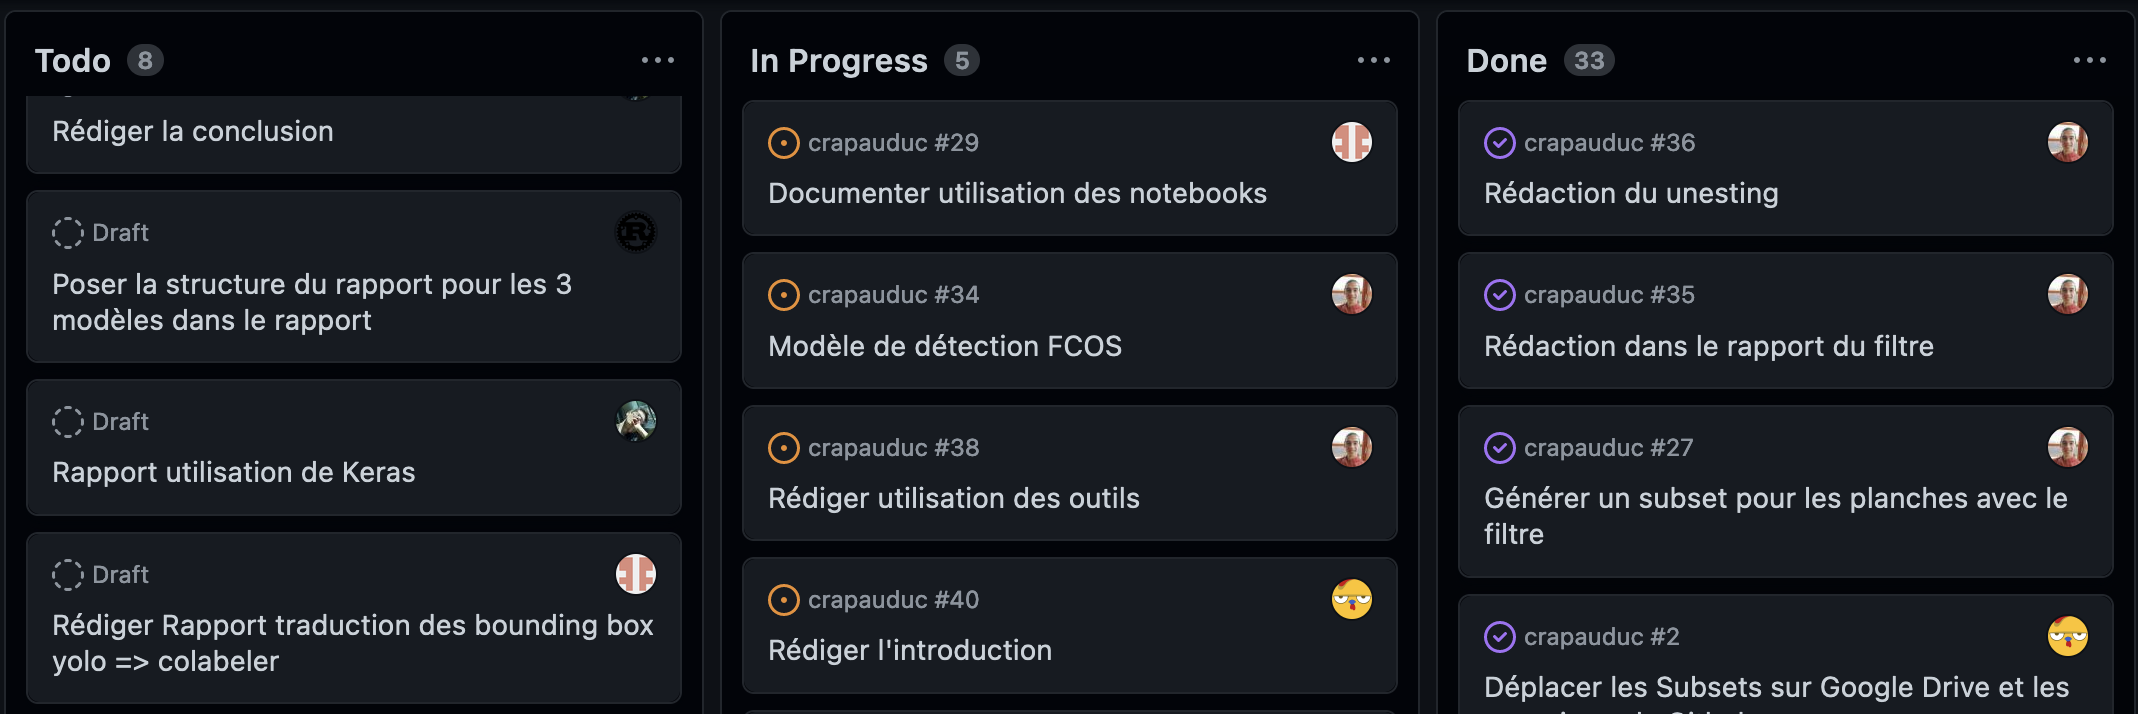
\includegraphics[width=0.8\linewidth]{images/kanban.png}
    \caption{Nos tâches du Kanban réparties en 3 catégories : à faire, en cours et terminées.}
    \label{fig:kanban}
\end{figure}

\chapter{Data preparation}

\section{Acquisition des données}

\paragraph*{Problème} Lors de ce projet, les données doivent être accessible à tous les membres et doivent être stockées de manière uniformisée pour faciliter le travail de groupe. Nous avons alors opté pour une structure regroupant les images par caméra et le nom de fichier correspondant est la date ISO standardisée de la date de la prise du fichier.

\paragraph*{Source} Nous avons récupéré un disque dur comprenant les 500GB dans le bureau de nos professeurs. La structure de fichier était partitionnée par caméra, année, jour, heure, minute. Cette structure était pratique pour naviguer dans les dossiers mais posait un problème pour extraire les informations car les métadonnées étaient stockées dans le path du fichier et non dans un fichier .csv externe. La nouvelle structure partitionnée par camera permet d'avoir toutes les images regroupées et ainsi d'avoir les métadonnées au même endroit. Nous avons ainsi écrit des scripts de transformations que l'on peut trouver dans le repository utils sur github.

\paragraph*{Format} Les images sont au format JPEG.

\paragraph*{Numéro de séquence} Une information qui n'était pas présente originellement était le numéro de séquence des images. Lorsque la caméra détectait un mouvement continu, la même action pouvait résulter sur plusieurs images différentes. Nous avons donc considéré une séquence valide si sur la même caméra, les images sont prise à la suite dans un interval de temps inférieur à 2 secondes. Ce numéro est ainsi ajouté aux métadonnées et permet de réaliser des analyses plus approfondies.

\section{Stockage des Données}

Afin de stocker les données, nous utilisons deux espaces de stockage différents. Premièrement, nous utilisons le serveur atlas mis à disposition pour stocker les images brutes. Deuxièmement, nous utilisons Google Drive pour stocker les subsets d'images traitées. De cette manière, nous avons une source de donnée fiable et pouvons ainsi tous travailler en parallèle avec les mêmes données uniformisées.

\paragraph*{Datalake}

Les données désarborisées ainsi que les données originales sont stockées sur le serveur atlas dans le dossier \texttt{/home/crapauduc/data/}. Ce dossier est accessible à tous les membres du groupe. Les images sont stockées dans des dossiers par caméra et le nom de fichier est la date ISO standardisée de la date de la prise du fichier.

\paragraph{Subsets}

Les subsets sont stockés dans le Google Drive et peuvent être utilisé pour tester//entraîner différents algorithmes




\chapter{Filtrage}

\paragraph*{Idée générale}
Le but de ce chapitre est de décrire les différentes méthodes de filtrage utilisées pour améliorer la qualité des données.

\paragraph*{Problème}
Le dataset original est composé de 18 caméras regroupant plus de 800'000 images. Une bonne partie de ces images sont des faux positifs. Il est donc nécessaire de filtrer les images afin de ne garder que les images qui nous intéressent. Une première observation nous fait remarquer que les images uniquement constituées de feuilles n'ont jamais d'animaux. Ensuite, une deuxième lecture nous fait remarquer que les animaux se déplacent plus facilement par temps humide. Et finalement, nous constatons que les animaux sont nombreux certains jours. À partir de ces observations, nous avons élaboré 3 méthodes pour filtrer les images et ainsi augmenter notre probabilité de trouver des animaux pour constituer de nouveaux labels ou constituer un dataset de validation.
Ces méthodes sont décrites dans les sections suivantes.

\section{Analyse de la météo}

\section{Analyse du nombre d'animaux}

\section{Détecteur de planches}

Nous avons développé un réseau de neurones convolutif à l'aide de la libraire PyTorch. Ce classificateur binaire, prédit ou non la présence de planche.

\paragraph*{Dataset d'entraînement}

Nous avons extrait 600 images d'une même caméra et labellisé 359 non planches et 241 planches. Ensuite, nous avons développé un dataloader permettant d'intégrer nos labels et de charger des batchs de données directement dans la libraire PyTorch. Celui ci, utilise un pipeline d'entrée qui applique plusieurs transformations à l'image avant de pouvoir l'utiliser comme un tenseur.

\begin{figure}[!htb]
    \centering
    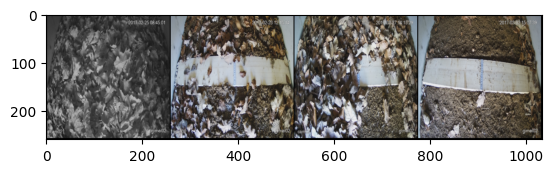
\includegraphics[width=200px]{images/filtre_exemple_data}
    \caption{Exemple de données d'entraînement}
    \label{fig:Entraînement du filtre}
\end{figure}

\paragraph*{Architecture du Détecteur}

Le détecteur est simplement constitué de 3 couches convolutives suivi de 2 couches entièrement connectées. Les channels d'entrée et de sortie des couches convolutives est de : 3 - 32, 32 - 64, 64 - 128. Le nombre de neurones des couches fully connected sont de 128 et 1 pour le neurone de sortie. La fonction de coût utilisé est la BCELoss et l'optimiseur est Adam. Le réseau est entraîné pendant 10 epochs avec un learning rate de 0.001 et un momentum de 0.9 sur 3 epochs.

\begin{figure}[!htb]
    \centering
    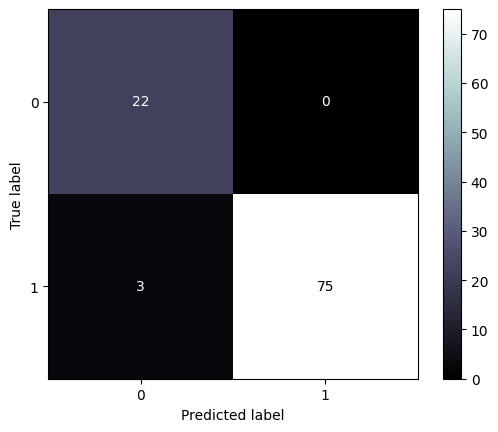
\includegraphics[width=200px]{images/filtre_cmatrix}
    \caption{Matrice de confusion du détecteur de planche}
    \label{fig:Matrice de confusion du filtre}
\end{figure}

\paragraph*{Résultats}

Le détecteur de planche a une précision de 1 et un recall de 0.98 sur la détection de planche. En revanche, la précision sur la détection de non planche est de 0.88 et un recall de 1. Ce qui veut dire que notre filtre est un peu trop efficace et a tendance à se tromper pour détecter les images sans planche. Comme les résultats sont satisfaisant pour dégrossir le travail, nous n'avons pas passé de temps supplémentaire à optimiser le réseau afin qu'il sépare mieux les images dotés d'une planche ou non. Comme, nous traitons une grande quantité de données, l'erreur est acceptable. Lancé sur la quasi intégralité du dataset, le filtre a tourné pendant plus de 10h sur un ordinateur de bureau doté d'un processeur Ryzen9500X. Au final, le filtre a détecté 48910 images de non planches sur les 754543 images analysées.
\chapter{Models}

\section{Model1}
\paragraph{description}
\subsection{Training}

\section{Model2}
\paragraph{description}
\subsection{Training}
\chapter{Evaluation}

\section{Section1}
\paragraph{paragraph1}
\subsection{Features}

Ceci est un acronyme \acl{kNN}
\chapter{Deployment}

\section{Section1}
\paragraph{paragraph1}
\subsection{Features}


\chapter{Conclusion}
Ceci est un acronyme \acl{kNN}

\end{document}
